\documentclass[tikz, border=1mm]{standalone}
\begin{document}
\begin{minipage}{\textwidth}
\centering
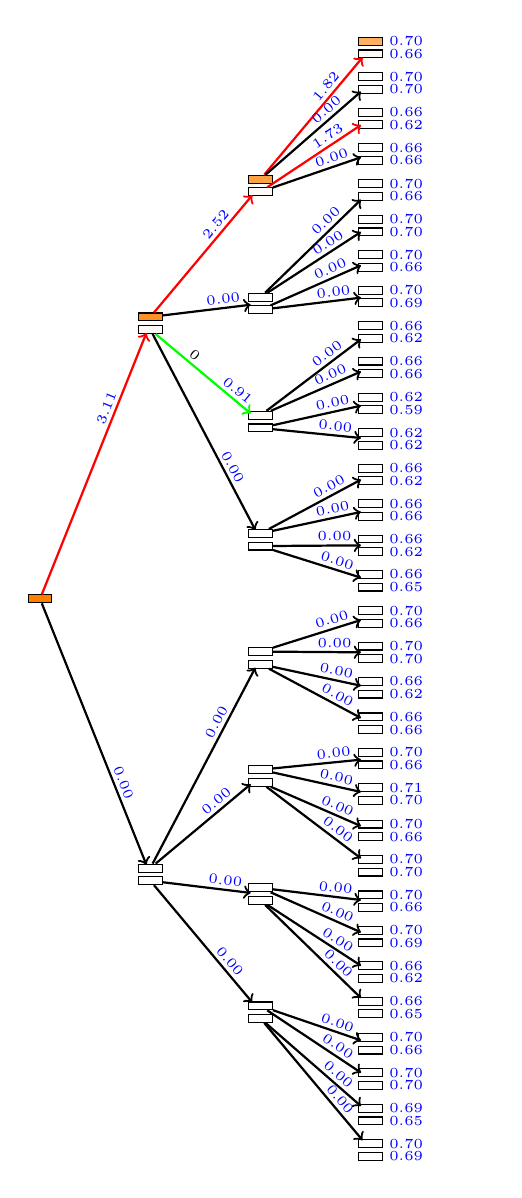
\begin{tikzpicture}
\tikzstyle{between} = [rectangle, draw=none]
\tikzstyle{qval}    = [rectangle, text centered, text width=2cm]
\node[between] at (-8.60, 3.50) (1_b_0){};
\node[between] at (-8.60, -3.50) (1_b_1){};
\node[between] at (-7.20, 5.25) (2_b_0){};
\node[between] at (-7.20, 3.75) (2_b_1){};
\node[between] at (-7.20, 2.25) (2_b_2){};
\node[between] at (-7.20, 0.75) (2_b_3){};
\node[between] at (-7.20, -0.75) (2_b_4){};
\node[between] at (-7.20, -2.25) (2_b_5){};
\node[between] at (-7.20, -3.75) (2_b_6){};
\node[between] at (-7.20, -5.25) (2_b_7){};
\node[between] at (-5.80, 7.00) (3_b_0){};
\node[between] at (-5.80, 6.55) (3_b_1){};
\node[between] at (-5.80, 6.10) (3_b_2){};
\node[between] at (-5.80, 5.65) (3_b_3){};
\node[between] at (-5.80, 5.19) (3_b_4){};
\node[between] at (-5.80, 4.74) (3_b_5){};
\node[between] at (-5.80, 4.29) (3_b_6){};
\node[between] at (-5.80, 3.84) (3_b_7){};
\node[between] at (-5.80, 3.39) (3_b_8){};
\node[between] at (-5.80, 2.94) (3_b_9){};
\node[between] at (-5.80, 2.48) (3_b_10){};
\node[between] at (-5.80, 2.03) (3_b_11){};
\node[between] at (-5.80, 1.58) (3_b_12){};
\node[between] at (-5.80, 1.13) (3_b_13){};
\node[between] at (-5.80, 0.68) (3_b_14){};
\node[between] at (-5.80, 0.23) (3_b_15){};
\node[between] at (-5.80, -0.23) (3_b_16){};
\node[between] at (-5.80, -0.68) (3_b_17){};
\node[between] at (-5.80, -1.13) (3_b_18){};
\node[between] at (-5.80, -1.58) (3_b_19){};
\node[between] at (-5.80, -2.03) (3_b_20){};
\node[between] at (-5.80, -2.48) (3_b_21){};
\node[between] at (-5.80, -2.94) (3_b_22){};
\node[between] at (-5.80, -3.39) (3_b_23){};
\node[between] at (-5.80, -3.84) (3_b_24){};
\node[between] at (-5.80, -4.29) (3_b_25){};
\node[between] at (-5.80, -4.74) (3_b_26){};
\node[between] at (-5.80, -5.19) (3_b_27){};
\node[between] at (-5.80, -5.65) (3_b_28){};
\node[between] at (-5.80, -6.10) (3_b_29){};
\node[between] at (-5.80, -6.55) (3_b_30){};
\node[between] at (-5.80, -7.00) (3_b_31){};
\node[rectangle, text centered, draw=black, minimum height=1mm, text width=3mm, inner sep=0pt, fill=orange, fill opacity=1.00, draw opacity=1] at (-10.00, 0.00) (0_s_0){};
\node[rectangle, text centered, draw=black, minimum height=1mm, text width=3mm, inner sep=0pt, fill=orange, fill opacity=0.86, draw opacity=1] at (-8.60, 3.58) (1_s_0) {};
\node[rectangle, text centered, draw=black, minimum height=1mm, text width=3mm, inner sep=0pt, fill=orange, fill opacity=0.04, draw opacity=1] at (-8.60, 3.42) (1_s_1) {};
\node[rectangle, text centered, draw=black, minimum height=1mm, text width=3mm, inner sep=0pt, fill=orange, fill opacity=0.00, draw opacity=1] at (-8.60, -3.42) (1_s_2) {};
\node[rectangle, text centered, draw=black, minimum height=1mm, text width=3mm, inner sep=0pt, fill=orange, fill opacity=0.00, draw opacity=1] at (-8.60, -3.58) (1_s_3) {};
\node[rectangle, text centered, draw=black, minimum height=1mm, text width=3mm, inner sep=0pt, fill=orange, fill opacity=0.74, draw opacity=1] at (-7.20, 5.33) (2_s_0) {};
\node[rectangle, text centered, draw=black, minimum height=1mm, text width=3mm, inner sep=0pt, fill=orange, fill opacity=0.04, draw opacity=1] at (-7.20, 5.17) (2_s_1) {};
\node[rectangle, text centered, draw=black, minimum height=1mm, text width=3mm, inner sep=0pt, fill=orange, fill opacity=0.00, draw opacity=1] at (-7.20, 3.83) (2_s_2) {};
\node[rectangle, text centered, draw=black, minimum height=1mm, text width=3mm, inner sep=0pt, fill=orange, fill opacity=0.00, draw opacity=1] at (-7.20, 3.67) (2_s_3) {};
\node[rectangle, text centered, draw=black, minimum height=1mm, text width=3mm, inner sep=0pt, fill=orange, fill opacity=0.03, draw opacity=1] at (-7.20, 2.33) (2_s_4) {};
\node[rectangle, text centered, draw=black, minimum height=1mm, text width=3mm, inner sep=0pt, fill=orange, fill opacity=0.00, draw opacity=1] at (-7.20, 2.17) (2_s_5) {};
\node[rectangle, text centered, draw=black, minimum height=1mm, text width=3mm, inner sep=0pt, fill=orange, fill opacity=0.00, draw opacity=1] at (-7.20, 0.83) (2_s_6) {};
\node[rectangle, text centered, draw=black, minimum height=1mm, text width=3mm, inner sep=0pt, fill=orange, fill opacity=0.00, draw opacity=1] at (-7.20, 0.67) (2_s_7) {};
\node[rectangle, text centered, draw=black, minimum height=1mm, text width=3mm, inner sep=0pt, fill=orange, fill opacity=0.00, draw opacity=1] at (-7.20, -0.67) (2_s_8) {};
\node[rectangle, text centered, draw=black, minimum height=1mm, text width=3mm, inner sep=0pt, fill=orange, fill opacity=0.00, draw opacity=1] at (-7.20, -0.83) (2_s_9) {};
\node[rectangle, text centered, draw=black, minimum height=1mm, text width=3mm, inner sep=0pt, fill=orange, fill opacity=0.00, draw opacity=1] at (-7.20, -2.17) (2_s_10) {};
\node[rectangle, text centered, draw=black, minimum height=1mm, text width=3mm, inner sep=0pt, fill=orange, fill opacity=0.00, draw opacity=1] at (-7.20, -2.33) (2_s_11) {};
\node[rectangle, text centered, draw=black, minimum height=1mm, text width=3mm, inner sep=0pt, fill=orange, fill opacity=0.00, draw opacity=1] at (-7.20, -3.67) (2_s_12) {};
\node[rectangle, text centered, draw=black, minimum height=1mm, text width=3mm, inner sep=0pt, fill=orange, fill opacity=0.00, draw opacity=1] at (-7.20, -3.83) (2_s_13) {};
\node[rectangle, text centered, draw=black, minimum height=1mm, text width=3mm, inner sep=0pt, fill=orange, fill opacity=0.00, draw opacity=1] at (-7.20, -5.17) (2_s_14) {};
\node[rectangle, text centered, draw=black, minimum height=1mm, text width=3mm, inner sep=0pt, fill=orange, fill opacity=0.00, draw opacity=1] at (-7.20, -5.33) (2_s_15) {};
\node[rectangle, text centered, draw=black, minimum height=1mm, text width=3mm, inner sep=0pt, fill=orange, fill opacity=0.63, draw opacity=1] at (-5.80, 7.08) (3_s_0) {};
\node[qval] at (-5.35, 7.08) () {\tiny \textcolor{blue}{0.70}};
\node[rectangle, text centered, draw=black, minimum height=1mm, text width=3mm, inner sep=0pt, fill=orange, fill opacity=0.03, draw opacity=1] at (-5.80, 6.92) (3_s_1) {};
\node[qval] at (-5.35, 6.92) () {\tiny \textcolor{blue}{0.66}};
\node[rectangle, text centered, draw=black, minimum height=1mm, text width=3mm, inner sep=0pt, fill=orange, fill opacity=0.00, draw opacity=1] at (-5.80, 6.63) (3_s_2) {};
\node[qval] at (-5.35, 6.63) () {\tiny \textcolor{blue}{0.70}};
\node[rectangle, text centered, draw=black, minimum height=1mm, text width=3mm, inner sep=0pt, fill=orange, fill opacity=0.00, draw opacity=1] at (-5.80, 6.47) (3_s_3) {};
\node[qval] at (-5.35, 6.47) () {\tiny \textcolor{blue}{0.70}};
\node[rectangle, text centered, draw=black, minimum height=1mm, text width=3mm, inner sep=0pt, fill=orange, fill opacity=0.03, draw opacity=1] at (-5.80, 6.18) (3_s_4) {};
\node[qval] at (-5.35, 6.18) () {\tiny \textcolor{blue}{0.66}};
\node[rectangle, text centered, draw=black, minimum height=1mm, text width=3mm, inner sep=0pt, fill=orange, fill opacity=0.00, draw opacity=1] at (-5.80, 6.02) (3_s_5) {};
\node[qval] at (-5.35, 6.02) () {\tiny \textcolor{blue}{0.62}};
\node[rectangle, text centered, draw=black, minimum height=1mm, text width=3mm, inner sep=0pt, fill=orange, fill opacity=0.00, draw opacity=1] at (-5.80, 5.73) (3_s_6) {};
\node[qval] at (-5.35, 5.73) () {\tiny \textcolor{blue}{0.66}};
\node[rectangle, text centered, draw=black, minimum height=1mm, text width=3mm, inner sep=0pt, fill=orange, fill opacity=0.00, draw opacity=1] at (-5.80, 5.57) (3_s_7) {};
\node[qval] at (-5.35, 5.57) () {\tiny \textcolor{blue}{0.66}};
\node[rectangle, text centered, draw=black, minimum height=1mm, text width=3mm, inner sep=0pt, fill=orange, fill opacity=0.00, draw opacity=1] at (-5.80, 5.27) (3_s_8) {};
\node[qval] at (-5.35, 5.27) () {\tiny \textcolor{blue}{0.70}};
\node[rectangle, text centered, draw=black, minimum height=1mm, text width=3mm, inner sep=0pt, fill=orange, fill opacity=0.00, draw opacity=1] at (-5.80, 5.11) (3_s_9) {};
\node[qval] at (-5.35, 5.11) () {\tiny \textcolor{blue}{0.66}};
\node[rectangle, text centered, draw=black, minimum height=1mm, text width=3mm, inner sep=0pt, fill=orange, fill opacity=0.00, draw opacity=1] at (-5.80, 4.82) (3_s_10) {};
\node[qval] at (-5.35, 4.82) () {\tiny \textcolor{blue}{0.70}};
\node[rectangle, text centered, draw=black, minimum height=1mm, text width=3mm, inner sep=0pt, fill=orange, fill opacity=0.00, draw opacity=1] at (-5.80, 4.66) (3_s_11) {};
\node[qval] at (-5.35, 4.66) () {\tiny \textcolor{blue}{0.70}};
\node[rectangle, text centered, draw=black, minimum height=1mm, text width=3mm, inner sep=0pt, fill=orange, fill opacity=0.00, draw opacity=1] at (-5.80, 4.37) (3_s_12) {};
\node[qval] at (-5.35, 4.37) () {\tiny \textcolor{blue}{0.70}};
\node[rectangle, text centered, draw=black, minimum height=1mm, text width=3mm, inner sep=0pt, fill=orange, fill opacity=0.00, draw opacity=1] at (-5.80, 4.21) (3_s_13) {};
\node[qval] at (-5.35, 4.21) () {\tiny \textcolor{blue}{0.66}};
\node[rectangle, text centered, draw=black, minimum height=1mm, text width=3mm, inner sep=0pt, fill=orange, fill opacity=0.00, draw opacity=1] at (-5.80, 3.92) (3_s_14) {};
\node[qval] at (-5.35, 3.92) () {\tiny \textcolor{blue}{0.70}};
\node[rectangle, text centered, draw=black, minimum height=1mm, text width=3mm, inner sep=0pt, fill=orange, fill opacity=0.00, draw opacity=1] at (-5.80, 3.76) (3_s_15) {};
\node[qval] at (-5.35, 3.76) () {\tiny \textcolor{blue}{0.69}};
\node[rectangle, text centered, draw=black, minimum height=1mm, text width=3mm, inner sep=0pt, fill=orange, fill opacity=0.01, draw opacity=1] at (-5.80, 3.47) (3_s_16) {};
\node[qval] at (-5.35, 3.47) () {\tiny \textcolor{blue}{0.66}};
\node[rectangle, text centered, draw=black, minimum height=1mm, text width=3mm, inner sep=0pt, fill=orange, fill opacity=0.00, draw opacity=1] at (-5.80, 3.31) (3_s_17) {};
\node[qval] at (-5.35, 3.31) () {\tiny \textcolor{blue}{0.62}};
\node[rectangle, text centered, draw=black, minimum height=1mm, text width=3mm, inner sep=0pt, fill=orange, fill opacity=0.01, draw opacity=1] at (-5.80, 3.02) (3_s_18) {};
\node[qval] at (-5.35, 3.02) () {\tiny \textcolor{blue}{0.66}};
\node[rectangle, text centered, draw=black, minimum height=1mm, text width=3mm, inner sep=0pt, fill=orange, fill opacity=0.00, draw opacity=1] at (-5.80, 2.86) (3_s_19) {};
\node[qval] at (-5.35, 2.86) () {\tiny \textcolor{blue}{0.66}};
\node[rectangle, text centered, draw=black, minimum height=1mm, text width=3mm, inner sep=0pt, fill=orange, fill opacity=0.00, draw opacity=1] at (-5.80, 2.56) (3_s_20) {};
\node[qval] at (-5.35, 2.56) () {\tiny \textcolor{blue}{0.62}};
\node[rectangle, text centered, draw=black, minimum height=1mm, text width=3mm, inner sep=0pt, fill=orange, fill opacity=0.00, draw opacity=1] at (-5.80, 2.40) (3_s_21) {};
\node[qval] at (-5.35, 2.40) () {\tiny \textcolor{blue}{0.59}};
\node[rectangle, text centered, draw=black, minimum height=1mm, text width=3mm, inner sep=0pt, fill=orange, fill opacity=0.00, draw opacity=1] at (-5.80, 2.11) (3_s_22) {};
\node[qval] at (-5.35, 2.11) () {\tiny \textcolor{blue}{0.62}};
\node[rectangle, text centered, draw=black, minimum height=1mm, text width=3mm, inner sep=0pt, fill=orange, fill opacity=0.00, draw opacity=1] at (-5.80, 1.95) (3_s_23) {};
\node[qval] at (-5.35, 1.95) () {\tiny \textcolor{blue}{0.62}};
\node[rectangle, text centered, draw=black, minimum height=1mm, text width=3mm, inner sep=0pt, fill=orange, fill opacity=0.00, draw opacity=1] at (-5.80, 1.66) (3_s_24) {};
\node[qval] at (-5.35, 1.66) () {\tiny \textcolor{blue}{0.66}};
\node[rectangle, text centered, draw=black, minimum height=1mm, text width=3mm, inner sep=0pt, fill=orange, fill opacity=0.00, draw opacity=1] at (-5.80, 1.50) (3_s_25) {};
\node[qval] at (-5.35, 1.50) () {\tiny \textcolor{blue}{0.62}};
\node[rectangle, text centered, draw=black, minimum height=1mm, text width=3mm, inner sep=0pt, fill=orange, fill opacity=0.00, draw opacity=1] at (-5.80, 1.21) (3_s_26) {};
\node[qval] at (-5.35, 1.21) () {\tiny \textcolor{blue}{0.66}};
\node[rectangle, text centered, draw=black, minimum height=1mm, text width=3mm, inner sep=0pt, fill=orange, fill opacity=0.00, draw opacity=1] at (-5.80, 1.05) (3_s_27) {};
\node[qval] at (-5.35, 1.05) () {\tiny \textcolor{blue}{0.66}};
\node[rectangle, text centered, draw=black, minimum height=1mm, text width=3mm, inner sep=0pt, fill=orange, fill opacity=0.00, draw opacity=1] at (-5.80, 0.76) (3_s_28) {};
\node[qval] at (-5.35, 0.76) () {\tiny \textcolor{blue}{0.66}};
\node[rectangle, text centered, draw=black, minimum height=1mm, text width=3mm, inner sep=0pt, fill=orange, fill opacity=0.00, draw opacity=1] at (-5.80, 0.60) (3_s_29) {};
\node[qval] at (-5.35, 0.60) () {\tiny \textcolor{blue}{0.62}};
\node[rectangle, text centered, draw=black, minimum height=1mm, text width=3mm, inner sep=0pt, fill=orange, fill opacity=0.00, draw opacity=1] at (-5.80, 0.31) (3_s_30) {};
\node[qval] at (-5.35, 0.31) () {\tiny \textcolor{blue}{0.66}};
\node[rectangle, text centered, draw=black, minimum height=1mm, text width=3mm, inner sep=0pt, fill=orange, fill opacity=0.00, draw opacity=1] at (-5.80, 0.15) (3_s_31) {};
\node[qval] at (-5.35, 0.15) () {\tiny \textcolor{blue}{0.65}};
\node[rectangle, text centered, draw=black, minimum height=1mm, text width=3mm, inner sep=0pt, fill=orange, fill opacity=0.00, draw opacity=1] at (-5.80, -0.15) (3_s_32) {};
\node[qval] at (-5.35, -0.15) () {\tiny \textcolor{blue}{0.70}};
\node[rectangle, text centered, draw=black, minimum height=1mm, text width=3mm, inner sep=0pt, fill=orange, fill opacity=0.00, draw opacity=1] at (-5.80, -0.31) (3_s_33) {};
\node[qval] at (-5.35, -0.31) () {\tiny \textcolor{blue}{0.66}};
\node[rectangle, text centered, draw=black, minimum height=1mm, text width=3mm, inner sep=0pt, fill=orange, fill opacity=0.00, draw opacity=1] at (-5.80, -0.60) (3_s_34) {};
\node[qval] at (-5.35, -0.60) () {\tiny \textcolor{blue}{0.70}};
\node[rectangle, text centered, draw=black, minimum height=1mm, text width=3mm, inner sep=0pt, fill=orange, fill opacity=0.00, draw opacity=1] at (-5.80, -0.76) (3_s_35) {};
\node[qval] at (-5.35, -0.76) () {\tiny \textcolor{blue}{0.70}};
\node[rectangle, text centered, draw=black, minimum height=1mm, text width=3mm, inner sep=0pt, fill=orange, fill opacity=0.00, draw opacity=1] at (-5.80, -1.05) (3_s_36) {};
\node[qval] at (-5.35, -1.05) () {\tiny \textcolor{blue}{0.66}};
\node[rectangle, text centered, draw=black, minimum height=1mm, text width=3mm, inner sep=0pt, fill=orange, fill opacity=0.00, draw opacity=1] at (-5.80, -1.21) (3_s_37) {};
\node[qval] at (-5.35, -1.21) () {\tiny \textcolor{blue}{0.62}};
\node[rectangle, text centered, draw=black, minimum height=1mm, text width=3mm, inner sep=0pt, fill=orange, fill opacity=0.00, draw opacity=1] at (-5.80, -1.50) (3_s_38) {};
\node[qval] at (-5.35, -1.50) () {\tiny \textcolor{blue}{0.66}};
\node[rectangle, text centered, draw=black, minimum height=1mm, text width=3mm, inner sep=0pt, fill=orange, fill opacity=0.00, draw opacity=1] at (-5.80, -1.66) (3_s_39) {};
\node[qval] at (-5.35, -1.66) () {\tiny \textcolor{blue}{0.66}};
\node[rectangle, text centered, draw=black, minimum height=1mm, text width=3mm, inner sep=0pt, fill=orange, fill opacity=0.00, draw opacity=1] at (-5.80, -1.95) (3_s_40) {};
\node[qval] at (-5.35, -1.95) () {\tiny \textcolor{blue}{0.70}};
\node[rectangle, text centered, draw=black, minimum height=1mm, text width=3mm, inner sep=0pt, fill=orange, fill opacity=0.00, draw opacity=1] at (-5.80, -2.11) (3_s_41) {};
\node[qval] at (-5.35, -2.11) () {\tiny \textcolor{blue}{0.66}};
\node[rectangle, text centered, draw=black, minimum height=1mm, text width=3mm, inner sep=0pt, fill=orange, fill opacity=0.00, draw opacity=1] at (-5.80, -2.40) (3_s_42) {};
\node[qval] at (-5.35, -2.40) () {\tiny \textcolor{blue}{0.71}};
\node[rectangle, text centered, draw=black, minimum height=1mm, text width=3mm, inner sep=0pt, fill=orange, fill opacity=0.00, draw opacity=1] at (-5.80, -2.56) (3_s_43) {};
\node[qval] at (-5.35, -2.56) () {\tiny \textcolor{blue}{0.70}};
\node[rectangle, text centered, draw=black, minimum height=1mm, text width=3mm, inner sep=0pt, fill=orange, fill opacity=0.00, draw opacity=1] at (-5.80, -2.86) (3_s_44) {};
\node[qval] at (-5.35, -2.86) () {\tiny \textcolor{blue}{0.70}};
\node[rectangle, text centered, draw=black, minimum height=1mm, text width=3mm, inner sep=0pt, fill=orange, fill opacity=0.00, draw opacity=1] at (-5.80, -3.02) (3_s_45) {};
\node[qval] at (-5.35, -3.02) () {\tiny \textcolor{blue}{0.66}};
\node[rectangle, text centered, draw=black, minimum height=1mm, text width=3mm, inner sep=0pt, fill=orange, fill opacity=0.00, draw opacity=1] at (-5.80, -3.31) (3_s_46) {};
\node[qval] at (-5.35, -3.31) () {\tiny \textcolor{blue}{0.70}};
\node[rectangle, text centered, draw=black, minimum height=1mm, text width=3mm, inner sep=0pt, fill=orange, fill opacity=0.00, draw opacity=1] at (-5.80, -3.47) (3_s_47) {};
\node[qval] at (-5.35, -3.47) () {\tiny \textcolor{blue}{0.70}};
\node[rectangle, text centered, draw=black, minimum height=1mm, text width=3mm, inner sep=0pt, fill=orange, fill opacity=0.00, draw opacity=1] at (-5.80, -3.76) (3_s_48) {};
\node[qval] at (-5.35, -3.76) () {\tiny \textcolor{blue}{0.70}};
\node[rectangle, text centered, draw=black, minimum height=1mm, text width=3mm, inner sep=0pt, fill=orange, fill opacity=0.00, draw opacity=1] at (-5.80, -3.92) (3_s_49) {};
\node[qval] at (-5.35, -3.92) () {\tiny \textcolor{blue}{0.66}};
\node[rectangle, text centered, draw=black, minimum height=1mm, text width=3mm, inner sep=0pt, fill=orange, fill opacity=0.00, draw opacity=1] at (-5.80, -4.21) (3_s_50) {};
\node[qval] at (-5.35, -4.21) () {\tiny \textcolor{blue}{0.70}};
\node[rectangle, text centered, draw=black, minimum height=1mm, text width=3mm, inner sep=0pt, fill=orange, fill opacity=0.00, draw opacity=1] at (-5.80, -4.37) (3_s_51) {};
\node[qval] at (-5.35, -4.37) () {\tiny \textcolor{blue}{0.69}};
\node[rectangle, text centered, draw=black, minimum height=1mm, text width=3mm, inner sep=0pt, fill=orange, fill opacity=0.00, draw opacity=1] at (-5.80, -4.66) (3_s_52) {};
\node[qval] at (-5.35, -4.66) () {\tiny \textcolor{blue}{0.66}};
\node[rectangle, text centered, draw=black, minimum height=1mm, text width=3mm, inner sep=0pt, fill=orange, fill opacity=0.00, draw opacity=1] at (-5.80, -4.82) (3_s_53) {};
\node[qval] at (-5.35, -4.82) () {\tiny \textcolor{blue}{0.62}};
\node[rectangle, text centered, draw=black, minimum height=1mm, text width=3mm, inner sep=0pt, fill=orange, fill opacity=0.00, draw opacity=1] at (-5.80, -5.11) (3_s_54) {};
\node[qval] at (-5.35, -5.11) () {\tiny \textcolor{blue}{0.66}};
\node[rectangle, text centered, draw=black, minimum height=1mm, text width=3mm, inner sep=0pt, fill=orange, fill opacity=0.00, draw opacity=1] at (-5.80, -5.27) (3_s_55) {};
\node[qval] at (-5.35, -5.27) () {\tiny \textcolor{blue}{0.65}};
\node[rectangle, text centered, draw=black, minimum height=1mm, text width=3mm, inner sep=0pt, fill=orange, fill opacity=0.00, draw opacity=1] at (-5.80, -5.57) (3_s_56) {};
\node[qval] at (-5.35, -5.57) () {\tiny \textcolor{blue}{0.70}};
\node[rectangle, text centered, draw=black, minimum height=1mm, text width=3mm, inner sep=0pt, fill=orange, fill opacity=0.00, draw opacity=1] at (-5.80, -5.73) (3_s_57) {};
\node[qval] at (-5.35, -5.73) () {\tiny \textcolor{blue}{0.66}};
\node[rectangle, text centered, draw=black, minimum height=1mm, text width=3mm, inner sep=0pt, fill=orange, fill opacity=0.00, draw opacity=1] at (-5.80, -6.02) (3_s_58) {};
\node[qval] at (-5.35, -6.02) () {\tiny \textcolor{blue}{0.70}};
\node[rectangle, text centered, draw=black, minimum height=1mm, text width=3mm, inner sep=0pt, fill=orange, fill opacity=0.00, draw opacity=1] at (-5.80, -6.18) (3_s_59) {};
\node[qval] at (-5.35, -6.18) () {\tiny \textcolor{blue}{0.70}};
\node[rectangle, text centered, draw=black, minimum height=1mm, text width=3mm, inner sep=0pt, fill=orange, fill opacity=0.00, draw opacity=1] at (-5.80, -6.47) (3_s_60) {};
\node[qval] at (-5.35, -6.47) () {\tiny \textcolor{blue}{0.69}};
\node[rectangle, text centered, draw=black, minimum height=1mm, text width=3mm, inner sep=0pt, fill=orange, fill opacity=0.00, draw opacity=1] at (-5.80, -6.63) (3_s_61) {};
\node[qval] at (-5.35, -6.63) () {\tiny \textcolor{blue}{0.65}};
\node[rectangle, text centered, draw=black, minimum height=1mm, text width=3mm, inner sep=0pt, fill=orange, fill opacity=0.00, draw opacity=1] at (-5.80, -6.92) (3_s_62) {};
\node[qval] at (-5.35, -6.92) () {\tiny \textcolor{blue}{0.70}};
\node[rectangle, text centered, draw=black, minimum height=1mm, text width=3mm, inner sep=0pt, fill=orange, fill opacity=0.00, draw opacity=1] at (-5.80, -7.08) (3_s_63) {};
\node[qval] at (-5.35, -7.08) () {\tiny \textcolor{blue}{0.69}};
\draw[->, thick, red] (0_s_0) -- (1_b_0) node [pos=0.70, above=-0.2em, sloped, font=\tiny] () {\textcolor{blue}{3.11}};
\draw[->, thick, black] (0_s_0) -- (1_b_1) node [pos=0.70, above=-0.2em, sloped, font=\tiny] () {\textcolor{blue}{0.00}};
\draw[->, thick, red] (1_s_0) -- (2_b_0) node [pos=0.70, above=-0.2em, sloped, font=\tiny] () {\textcolor{blue}{2.52}};
\draw[->, thick, black] (1_s_0) -- (2_b_1) node [pos=0.70, above=-0.2em, sloped, font=\tiny] () {\textcolor{blue}{0.00}};
\draw[->, thick, green] (1_s_1) -- (2_b_2) node [pos=0.35, above=-0.2em, sloped, font=\tiny] () {\textcolor{black}{0}} node [pos=0.80, above=-0.2em, sloped, font=\tiny] () {\textcolor{blue}{0.91}};
\draw[->, thick, black] (1_s_1) -- (2_b_3) node [pos=0.70, above=-0.2em, sloped, font=\tiny] () {\textcolor{blue}{0.00}};
\draw[->, thick, black] (1_s_2) -- (2_b_4) node [pos=0.70, above=-0.2em, sloped, font=\tiny] () {\textcolor{blue}{0.00}};
\draw[->, thick, black] (1_s_2) -- (2_b_5) node [pos=0.70, above=-0.2em, sloped, font=\tiny] () {\textcolor{blue}{0.00}};
\draw[->, thick, black] (1_s_3) -- (2_b_6) node [pos=0.70, above=-0.2em, sloped, font=\tiny] () {\textcolor{blue}{0.00}};
\draw[->, thick, black] (1_s_3) -- (2_b_7) node [pos=0.70, above=-0.2em, sloped, font=\tiny] () {\textcolor{blue}{0.00}};
\draw[->, thick, red] (2_s_0) -- (3_b_0) node [pos=0.70, above=-0.2em, sloped, font=\tiny] () {\textcolor{blue}{1.82}};
\draw[->, thick, black] (2_s_0) -- (3_b_1) node [pos=0.70, above=-0.2em, sloped, font=\tiny] () {\textcolor{blue}{0.00}};
\draw[->, thick, red] (2_s_1) -- (3_b_2) node [pos=0.70, above=-0.2em, sloped, font=\tiny] () {\textcolor{blue}{1.73}};
\draw[->, thick, black] (2_s_1) -- (3_b_3) node [pos=0.70, above=-0.2em, sloped, font=\tiny] () {\textcolor{blue}{0.00}};
\draw[->, thick, black] (2_s_2) -- (3_b_4) node [pos=0.70, above=-0.2em, sloped, font=\tiny] () {\textcolor{blue}{0.00}};
\draw[->, thick, black] (2_s_2) -- (3_b_5) node [pos=0.70, above=-0.2em, sloped, font=\tiny] () {\textcolor{blue}{0.00}};
\draw[->, thick, black] (2_s_3) -- (3_b_6) node [pos=0.70, above=-0.2em, sloped, font=\tiny] () {\textcolor{blue}{0.00}};
\draw[->, thick, black] (2_s_3) -- (3_b_7) node [pos=0.70, above=-0.2em, sloped, font=\tiny] () {\textcolor{blue}{0.00}};
\draw[->, thick, black] (2_s_4) -- (3_b_8) node [pos=0.70, above=-0.2em, sloped, font=\tiny] () {\textcolor{blue}{0.00}};
\draw[->, thick, black] (2_s_4) -- (3_b_9) node [pos=0.70, above=-0.2em, sloped, font=\tiny] () {\textcolor{blue}{0.00}};
\draw[->, thick, black] (2_s_5) -- (3_b_10) node [pos=0.70, above=-0.2em, sloped, font=\tiny] () {\textcolor{blue}{0.00}};
\draw[->, thick, black] (2_s_5) -- (3_b_11) node [pos=0.70, above=-0.2em, sloped, font=\tiny] () {\textcolor{blue}{0.00}};
\draw[->, thick, black] (2_s_6) -- (3_b_12) node [pos=0.70, above=-0.2em, sloped, font=\tiny] () {\textcolor{blue}{0.00}};
\draw[->, thick, black] (2_s_6) -- (3_b_13) node [pos=0.70, above=-0.2em, sloped, font=\tiny] () {\textcolor{blue}{0.00}};
\draw[->, thick, black] (2_s_7) -- (3_b_14) node [pos=0.70, above=-0.2em, sloped, font=\tiny] () {\textcolor{blue}{0.00}};
\draw[->, thick, black] (2_s_7) -- (3_b_15) node [pos=0.70, above=-0.2em, sloped, font=\tiny] () {\textcolor{blue}{0.00}};
\draw[->, thick, black] (2_s_8) -- (3_b_16) node [pos=0.70, above=-0.2em, sloped, font=\tiny] () {\textcolor{blue}{0.00}};
\draw[->, thick, black] (2_s_8) -- (3_b_17) node [pos=0.70, above=-0.2em, sloped, font=\tiny] () {\textcolor{blue}{0.00}};
\draw[->, thick, black] (2_s_9) -- (3_b_18) node [pos=0.70, above=-0.2em, sloped, font=\tiny] () {\textcolor{blue}{0.00}};
\draw[->, thick, black] (2_s_9) -- (3_b_19) node [pos=0.70, above=-0.2em, sloped, font=\tiny] () {\textcolor{blue}{0.00}};
\draw[->, thick, black] (2_s_10) -- (3_b_20) node [pos=0.70, above=-0.2em, sloped, font=\tiny] () {\textcolor{blue}{0.00}};
\draw[->, thick, black] (2_s_10) -- (3_b_21) node [pos=0.70, above=-0.2em, sloped, font=\tiny] () {\textcolor{blue}{0.00}};
\draw[->, thick, black] (2_s_11) -- (3_b_22) node [pos=0.70, above=-0.2em, sloped, font=\tiny] () {\textcolor{blue}{0.00}};
\draw[->, thick, black] (2_s_11) -- (3_b_23) node [pos=0.70, above=-0.2em, sloped, font=\tiny] () {\textcolor{blue}{0.00}};
\draw[->, thick, black] (2_s_12) -- (3_b_24) node [pos=0.70, above=-0.2em, sloped, font=\tiny] () {\textcolor{blue}{0.00}};
\draw[->, thick, black] (2_s_12) -- (3_b_25) node [pos=0.70, above=-0.2em, sloped, font=\tiny] () {\textcolor{blue}{0.00}};
\draw[->, thick, black] (2_s_13) -- (3_b_26) node [pos=0.70, above=-0.2em, sloped, font=\tiny] () {\textcolor{blue}{0.00}};
\draw[->, thick, black] (2_s_13) -- (3_b_27) node [pos=0.70, above=-0.2em, sloped, font=\tiny] () {\textcolor{blue}{0.00}};
\draw[->, thick, black] (2_s_14) -- (3_b_28) node [pos=0.70, above=-0.2em, sloped, font=\tiny] () {\textcolor{blue}{0.00}};
\draw[->, thick, black] (2_s_14) -- (3_b_29) node [pos=0.70, above=-0.2em, sloped, font=\tiny] () {\textcolor{blue}{0.00}};
\draw[->, thick, black] (2_s_15) -- (3_b_30) node [pos=0.70, above=-0.2em, sloped, font=\tiny] () {\textcolor{blue}{0.00}};
\draw[->, thick, black] (2_s_15) -- (3_b_31) node [pos=0.70, above=-0.2em, sloped, font=\tiny] () {\textcolor{blue}{0.00}};
\end{tikzpicture}
\end{minipage}
\end{document}